\newpage
\renewcommand{\floatpagefraction}{0.9}
\noindent
The appendix provides proofs and additional analysis in Appendices~\ref{app:proofs} and~\ref{app:additional_math}, evaluation details in Appendix~\ref{app:protocol}, and sentence-level prefix experiments in Appendix~\ref{app:sentence}.

\section{Proofs and finite-budget analysis}
\label{app:proofs}
\subsection{Proof of Theorem~\ref{thm:decomposition}}
Define the self-consistency continuation value at any history by backward recursion.
\[
 V_j^S(h)=\int V_{j+1}^S(h,u)K_j^S(du\mid h),\qquad
 V_J^S(h)=\ind\{\text{final vote in }h\text{ is correct}\}.
\]
The notation $(h,u)$ includes the deterministic bookkeeping after the next window. Under path-consistency, conditional expectation gives
\[
 \E_P[V_{j+1}^S(H_{j+1})-V_j^S(H_j)\mid H_j=h]=d_j(h).
\]
Taking expectations and summing over $j$ telescopes. The initial value is $A_S$ and the expected terminal value is $A_P$, proving Equation~\ref{eq:risk}. This argument needs only bounded measurable values and a finite horizon. It does not require independent windows, a binary answer distribution, or a correct selected prefix. Since $0\leq V_{j+1}^S\leq1$, the standard variational definition
\[
 \TV(P,Q)=\sup_{0\leq f\leq1}|\E_Pf-\E_Qf|
\]
implies $|d_j(h)|\leq\TV(K_j^P,K_j^S)$. The triangle inequality and the fact that two probabilities differ by at most one prove Equation~\ref{eq:tv}.

\paragraph{Scope for stopping controllers.}
The displayed result compares fixed-budget self-consistency and path-consistency. A stopping controller can be represented by an absorbing terminal state and padding to a common finite maximum horizon. Both the reference value and the reference transition kernel must then include that parent's stopping rule. This extension does not allow replacing a confidence-weighted parent's final vote by a majority vote while claiming to compare the same parent.

\subsection{Proof of Theorem~\ref{thm:plurality}}
Fix a competitor $a$. The differences $D_i=X_i(a)-\mu_i(a)$ are martingale differences. Conditional on $\mathcal F_{i-1}$, their values lie in an interval of width at most two, since $X_i(a)\in[-1,1]$. The conditional bounded-variable exponential inequality therefore gives
\[
 \E[\exp(-\lambda D_i)\mid\mathcal F_{i-1}]\leq\exp(\lambda^2/2),\quad \lambda>0.
\]
This inequality follows by the convex upper bound on the exponential between the two interval endpoints and maximizing over a zero-mean two-point distribution. Iterating conditional expectations yields
$\E\exp(-\lambda\sum_iD_i)\leq\exp(B\lambda^2/2)$.
If the correct answer fails to outvote $a$, then $\sum_iX_i(a)\leq0$. By the almost-sure lower bound on accumulated conditional means, this implies $\sum_iD_i\leq-\Gamma_a$. Markov's inequality now bounds its probability by
\[
 \exp(-\lambda\Gamma_a+B\lambda^2/2).
\]
Taking $\lambda=\Gamma_a/B$ gives $\exp(-\Gamma_a^2/(2B))$. If the final vote is incorrect or tied, at least one incorrect category has count no smaller than the correct category. Union-bounding these events proves the result. Voting failure is covered by the union of competitor events.

\paragraph{What the assumption rules out.}
An unconditional gap $P(A_i=a^\star)>P(A_i=a)$ is insufficient. Conditioning on an early misleading prefix may reverse the gap, violating the almost-sure lower bound. Similarly, the observed mode need not equal $a^\star$. The Beta gate operates on the mode, whereas the theorem refers to the externally defined correct answer. An empirical evaluation of the assumption needs correctness information and conditional resampling beyond the current trajectories.

\subsection{Exact binary illustration without Taylor expansion}
For comparison with a single-promotion analysis, suppose $n$ root answers are independent Bernoulli with correctness probability $p_0$, and the remaining $r=B-n$ answers are conditionally independent with correctness probability $q_k$ after observing $k$ correct root answers. Fix a tie-as-failure convention. Define
\[
 Q_r(p,t)=\sum_{j=\max(0,t)}^r \binom{r}{j}p^j(1-p)^{r-j},
\]
with $Q_r(p,t)=0$ for $t>r$ and $Q_r(p,t)=1$ for $t\leq0$. Then
\begin{align}
 A_{\mathrm{PC}}&=\sum_{k=0}^{n}\binom{n}{k}p_0^k(1-p_0)^{n-k}
       Q_r(q_k,\lfloor B/2\rfloor+1-k),\label{eq:exactbinary}\\
 A_{\mathrm{SC}}&=Q_B(p_0,\lfloor B/2\rfloor+1).
\end{align}
Both parts contribute to the final vote. A gate that does not promote sets $q_k=p_0$ for that history. The formula is exact for this idealized model, including its tie convention; it is not a model of all levels of path-consistency.

For a concrete failure construction take $B=32,n=4,p_0=0.6,C=0.8$. If the four root answers are all wrong, their agreement score is $1-2^{-5}=0.96875$. Let the selected wrong prefix force all subsequent answers to be wrong ($q_0=0$), while all other histories retain $q_k=0.6$. The accuracy loss relative to self-consistency is exactly
\[
 (0.4)^4 Q_{28}(0.6,17)>0.
\]
Numerically, self-consistency accuracy in this construction is 0.835203095 and the intervention accuracy is 0.821096895, a loss of 1.41 percentage points. Thus even a model whose unprefixed correctness probability exceeds one half can be harmed by a gate-passing prefix. The construction does not assume symmetric beneficial and harmful effects. That symmetry is an additional modeling assumption, not an inference-time property. More generally, a consensus-only controller has no access to the sign of a prefix's correctness effect.

\subsection{Shared-prefix dependence}
Let a random shared prefix $Z$ induce correctness probability $p_Z$, and let $Y_1,Y_2$ be correctness indicators of two suffixes that are conditionally independent given $Z$. Then $\E[Y_1Y_2\mid Z]=p_Z^2$ and $\E Y_i=\E p_Z$, so
\begin{equation}
 \operatorname{Cov}(Y_1,Y_2)=\operatorname{Var}(p_Z).
 \label{eq:dependence}
\end{equation}
For a window of size $m$ with exchangeable correctness indicators, marginal correctness probability $\bar p$, and pairwise correlation $\rho$, summing variances and covariances gives
\[
 \operatorname{Var}(\bar Y)=\frac{\bar p(1-\bar p)}{m}[1+(m-1)\rho].
\]
For $0<\bar p<1$ and a positive variance inflation factor, this corresponds to $m/[1+(m-1)\rho]$ independent Bernoulli observations with the same variance. This conditional-mixture illustration is not an estimate of the effective sample size of a full path-consistency run. Neither that value nor a plug-in correction is used to calibrate the actual path-consistency gate.

\section{Additional analysis of prefix reuse}
\label{app:additional_math}
The following results clarify when prefix reuse can affect the final vote and how shared prefixes change the relationship between trajectory accuracy and voting accuracy.

\subsection{When can later windows still change the vote?}
Let $c_a$ count all valid votes for answer $a$ already generated, including votes from rejected windows. Let $\ell$ be a unique current leader and let $r$ be an upper bound on the number of answers still to be generated. Include an unseen competitor with count zero when defining $c_{(2)}=\max_{a\ne\ell}c_a$. Each remaining trajectory supplies at most one unit vote, and earlier votes cannot be removed or reweighted.

\begin{proposition}[Irreversible plurality]
\label{prop:lock}
If $c_\ell-c_{(2)}>r$, then $\ell$ is the unique final plurality winner for every possible continuation, including adaptive and dependent continuations. If $c_\ell-c_{(2)}<r$, a continuation assigning every remaining vote to a strongest competitor can overturn the leader. At equality a competitor can tie, so the outcome depends on the fixed tie rule.
\end{proposition}
\begin{proof}
For any competitor, the largest possible increase in its count relative to the leader is $r$. Thus its final deficit is at least $c_\ell-c_a-r$. A strictly positive minimum guarantees the leader remains unique. Conversely, giving all $r$ votes to a strongest competitor realizes that maximum increase, proving the remaining statements. Invalid outputs can only reduce the number of added votes and cannot break the sufficient condition.
\end{proof}

The statement concerns the realized vote, not correctness. Once a wrong leader is locked, a rollback cannot repair the final answer under this aggregation rule. Once a correct leader is locked, later prefixes cannot change final correctness either. For a fixed $B=32,m=4$, one may test the sufficient condition after window $j$ using $r=32-4j$. This is a diagnostic of the final vote, not a stopping rule used in the experiments. The condition says only that later votes cannot alter the outcome; it does not undo any effect of earlier prefixes on the current counts.

There is also a useful consequence for Theorem~\ref{thm:decomposition}. On a locked history, $V^S$ is constant over all admissible next windows, so $d_j(h)=0$. Accordingly,
\[
 |A_P-A_S|\leq\min\left\{1,\sum_j\E_P\left[
 \ind\{H_j\text{ is not locked}\}\,
 \TV(K_j^P(\cdot\mid H_j),K_j^S(\cdot\mid H_j))\right]\right\}.
\]
This refinement localizes possible final-vote effects to histories where future votes can still matter. It does not assert that unlocked histories are recoverable under the model's actual support, nor that their increments are favorable.

\subsection{Higher marginal correctness can yield a worse majority}
For a binary illustration, condition on a history with $n$ earlier votes, $k$ of them correct, and $r=B-n$ remaining votes. A random shared prefix $Z$ induces a correctness probability $p_Z$; conditional on $Z$ and the history, the remaining answers are independent Bernoulli variables. With ties counted as failures, let $t=\lfloor B/2\rfloor+1-k$. Using the binomial tail from Equation~\ref{eq:exactbinary}, the conditional final success probability is
\begin{equation}
 A_{\mathrm{shared}}(h)=\E[Q_r(p_Z,t)\mid h].
 \label{eq:mixturevote}
\end{equation}
If an independent prefix were instead drawn for each remaining answer under this stylized model, the probability would be $Q_r(\bar p,t)$, where $\bar p=\E[p_Z\mid h]$. These two expressions generally differ even at identical marginal correctness. Independent-prefix resampling here is an analytical comparator, not an evaluated path-consistency variant.

\begin{proposition}[Curvature of the voting response]
For $1\leq t\leq r$ and $0<p<1$,
\[
 \frac{d Q_r(p,t)}{dp}
 =r\binom{r-1}{t-1}p^{t-1}(1-p)^{r-t},
\]
and the sign of its second derivative is the sign of
$(t-1)-(r-1)p$. Thus $Q_r$ is concave above $p=(t-1)/(r-1)$ and convex below it when $r>1$. If the support of $p_Z$ lies wholly in the concave region, sharing cannot improve the voting probability relative to independent resampling at the same mean; in the convex region the inequality reverses.
\end{proposition}
\begin{proof}
Differentiate the finite binomial sum. Adjacent terms cancel, leaving the stated first derivative. Its logarithmic derivative is $(t-1)/p-(r-t)/(1-p)$, which has the stated sign. Jensen's inequality on either curvature region gives the comparison. For $r=1$ the response is linear. For $t\leq0$ or $t>r$ it is constant. When the support crosses the inflection point, these local curvature statements imply no universal ordering.
\end{proof}

For a finite-budget counterexample retaining the root votes, take four independent root answers with correctness probability 0.6 and 28 later answers sharing a latent prefix. Independently of the root, let $p_Z=1$ with probability 0.65 and $p_Z=0$ otherwise. The final vote is correct exactly when $p_Z=1$, hence its accuracy is 0.65. In contrast, 32 independent answers with correctness probability 0.6 succeed with probability $Q_{32}(0.6,17)=0.835203095$. Every later answer in the shared construction has higher marginal correctness (0.65 versus 0.6), and the mean across all 32 is 0.64375, yet its majority is worse. This deliberately extreme mixture is not a fitted path-consistency model or an assertion that these prefixes occur in the experiments. It demonstrates why per-trajectory correctness and agreement alone do not identify the accuracy of a shared-prefix vote.


\subsection{Agreement thresholds under a fixed answer distribution}
\label{app:gate_analysis}
A fixed-distribution calculation helps distinguish evidence for answer concentration from evidence for correctness. Suppose $n$ answers are sampled independently from one distribution with correct-answer probability $q$. For $1/2<C<1$, define
\[
 k_C(n)=\min\{k\in\{0,\ldots,n\}:c(n,k)\geq C\},
\]
taking $k_C(n)=n+1$ when the set is empty. The score in Equation~\ref{eq:beta} is increasing in $k$, and $k_C(n)>n/2$. Hence the correct answer passes the gate exactly when its count reaches $k_C(n)$, with probability
\[
 \Prb(\text{correct answer passes})=Q_n(q,k_C(n)).
\]
This expression concerns the source answer, not the semantic correctness of every token in its prefix.

An incorrect answer can pass only if the total number of incorrect answers is at least $k_C(n)$. Therefore
\[
 \Prb(\text{an incorrect answer passes})
 \leq Q_n(1-q,k_C(n)).
\]
Equality holds when all incorrect probability mass is concentrated on one alternative. This identifies a worst-case error distribution for a single fixed-distribution check. Raising $C$ increases the required count and reduces both correct and incorrect gate-passing probabilities at that check. In particular, a majority of correct answers can still fail a stringent gate, so the probability of failing to pass cannot be bounded solely by the probability of lacking a correct majority.

Successive checks in path-consistency reuse observations and change the sampling distribution. Their error probabilities therefore cannot be multiplied as if the checks were independent. More generally, if the conditional probability of an incorrect gate-passing decision at check $j$, given its preceding history, is bounded by $\varepsilon_j$, the probability of any such decision is at most $\sum_j\varepsilon_j$ by a union bound and conditional expectation. The gate itself does not establish these conditional bounds. The adaptive analysis in Section~\ref{sec:theory} avoids treating repeated agreement as a correctness guarantee.

\section{Method and evaluation details}
\label{app:algorithm}
\label{app:protocol}
\subsection{Window transitions and answer aggregation}
Table~\ref{tab:state_transitions} summarizes the controller in Section~\ref{sec:method}. The admitted set $\mathcal V$ controls prefix proposals and validation, whereas the final vote uses all valid completed answers. Answers from previously accepted windows remain in $\mathcal V$ after rollback.

\begin{table}[!htbp]
\centering\small
\caption{Prefix updates at window boundaries. Every valid completed answer remains eligible for final aggregation.}
\label{tab:state_transitions}
\begin{tabularx}{\linewidth}{@{}lXX@{}}
\toprule
State & Observation & Update\\
\midrule
Root & Valid answers available & Add answers to $\mathcal V$; propose an extension if the gate passes and a candidate exists.\\
Trial & Same modal answer and $c\geq C$ & Commit the prefix, admit answers, clear the failure count, and consider the next extension.\\
Trial & Modal answer changes or $c<C$ & Discard the proposal, return to the committed prefix, and increment the failure count.\\
Committed & Same modal answer and $c\geq C$ & Retain the prefix, admit answers, clear the failure count, and consider the next extension.\\
Committed & Modal answer changes or $c<C$ & Roll back one level and increment the failure count.\\
Any prefix & Two consecutive failures & Clear the prefix and disable further reuse for this question.\\
\bottomrule
\end{tabularx}
\end{table}

Failed windows provide neither admitted answers nor new prefix candidates. A failed candidate is not permanently excluded from all later source pools. When combined with an early-stopping method, sampling ends at a completed window according to that method's stopping rule, and its aggregation rule is retained.

\subsection{Datasets and prompting}
% Citations needed for the datasets and their official evaluation protocols.
We use the GSM8K test split, MATH-500, AIME 2024, AIME 2025, and GPQA-Diamond. GPQA option order is shuffled deterministically with seed 2027.

The mathematical reasoning instruction is \emph{Please reason step by step, and put your final answer within \texttt{\textbackslash boxed\{\}}.} GPQA presents four labeled options and requests the correct option letter in the same format. Llama uses its chat template. DeepSeek and Qwen use thinking mode, with the decoding settings in Section~\ref{sec:setup}. These interfaces differ, so comparisons are made within each model and dataset.

\subsection{Token and time accounting}
\label{app:accounting}
At an empty prefix, path-consistency reuses the corresponding self-consistency window, including after a return to root. Its original token count and generation time are charged in full. Windows with nonempty prefixes generate new continuations, and failed windows are also counted.

Let $T_{ij}$ and $G_{ij}$ be generated tokens and generation time for window $j$ of question $i$. Over $n$ questions, the means are
\[
 \bar T=\frac{1}{n}\sum_{i,j}T_{ij},\qquad
 \bar G=\frac{1}{n}\sum_{i,j}G_{ij}.
\]
Token savings are $1-\bar T_{\mathrm{PC}}/\bar T_{\mathrm{SC}}$, and a generation speed ratio is $\bar G_{\mathrm{SC}}/\bar G_{\mathrm{PC}}$. Tables with negative Save entries instead display the signed relative token change. A nominal prefix fraction is not a measured saving because continuation lengths can change. These measurements do not include all input-processing and orchestration costs or establish peak-memory and API-billing savings.

\subsection{Ablation settings}
\label{app:ablation_design}
The prefix-selection and recovery ablation fixes the 490 DeepSeek/MATH-500 evaluated questions, self-consistency root windows, source eligibility, prefix-length grid, and decoding settings. Accuracy additionally counts ten held-out engineering items as correct ($n=500$). Uniform selection samples from the same eligible candidates. Disabling recovery retains the active prefix after failure and disables the two-failure reset, while failed-window answers remain excluded from $\mathcal V$. All valid answers still enter the final vote. This removes the recovery mechanism as a whole rather than isolating a single rollback operation.

The full configuration and the three alternatives in Table~\ref{tab:selrec} have 438, 436, 433, and 433 correct answers out of 500. Relative to the full configuration, the alternatives have paired gains/losses of 3/5, 4/9, and 5/10. These single-run differences describe the observed contribution of each component rather than establishing its variability across repeated runs.

\paragraph{Agreement threshold.}
\label{app:threshold}
Table~\ref{tab:threshold} compares $C\in\{0,0.7,0.8,1\}$ on DeepSeek/GSM8K. At $C=0$, the gate imposes no minimum agreement score, but a valid modal answer and feasible prefix are still required. At $C=1$, prefix reuse is disabled. Lower values favor token savings, while higher values make reuse more conservative and favor accuracy preservation. The default remains $C=0.8$; this sensitivity analysis does not identify a universally optimal threshold.

\paragraph{Prefix length at a fixed history.}
\label{app:length_intervention}
A supplementary DeepSeek/MATH-500 study fixes the first-window history and the source chosen by local confidence selection, then varies the retained fraction over $\{0,0.2,0.4,0.6,0.8\}$. It covers 466 questions with feasible prefixes at every level and eight repetitions of a four-answer window per level. Of the remaining questions, 19 do not pass the initial gate and five lack a feasible endpoint. The final-vote diagnostic combines the intervened window with the same four root answers and 24 unprefixed answers. It therefore isolates one window under a fixed continuation, rather than estimating the full continuation expectation in Equation~\ref{eq:risk}. This analysis does not change the fixed prefix-length grid used at inference time.


\section{Initial exploration of sentence-level prefix reuse}
\label{app:sentence}
Before developing the current method, we first explored a sentence-level form of path-consistency for short-chain reasoning. The idea was to reuse complete early reasoning steps rather than generate every trajectory from scratch. This initial approach achieved substantial token savings with generally comparable accuracy on several arithmetic, commonsense, and symbolic tasks, motivating the controlled prefix reuse developed in Section~\ref{sec:method}. We summarize these earlier experiments and the insights they provided below.

The sentence-level approach samples 20 trajectories and randomly selects from eligible prefix candidates ending at sentence boundaries. Its default schedule allows three extension levels, with updates after every five trajectories. Unlike the current method, it does not use one shared prefix per window, the token-fraction grid, or the same trial-and-recovery controller. The results therefore characterize this initial approach and are not pooled with the main experiments.

The Llama-3-8B experiments use temperature 0.6, top-$p=0.9$, few-shot reasoning prompts, and an RTX 3090. Here a prefix level counts retained reasoning steps rather than a fraction of trajectory tokens. Comparisons retain their own self-consistency baselines and timing conventions. Reported speedup percentages denote the increase in speed relative to the corresponding baseline, not the percentage reduction in elapsed time.
% Source: paper/NIPS/04_evaluation.tex, Experimental Setting.
% Citation placeholders for Llama-3, Mistral, DeepSeek-V3, Llama-3.2, datasets, and baseline methods.

\subsection{Arithmetic, commonsense, and symbolic reasoning}
Table~\ref{tab:sentence_tasks} reports our initial results across ten short-chain reasoning tasks~\citep{cobbe2021training, patel2021nlp, miao2020diverse, roy2015solving,geva2021did,suzgun-etal-2023-challenging}. Sentence-level reuse reduces token generation across all tasks and thresholds, with savings ranging from 4.7\% to 36.6\%. Arithmetic accuracy is generally close to or above the self-consistency baseline. At $C=0.8$, GSM8K and Tracking Shuffled Objects improve by 3.7 and 5.2 percentage points, respectively, while Ruin Names and Logical Deduction decline. These results established the practical potential of prefix reuse while showing that its accuracy effects depend on the task.

\begin{table}[!htbp]
\centering\small
\caption{Sentence-level prefix reuse with Llama-3-8B. Each PC entry gives accuracy (\%) / token saving (\%) relative to its SC baseline. These results use the supplementary 20-trajectory setting.}
\label{tab:sentence_tasks}
\setlength{\tabcolsep}{4pt}
\begin{tabular}{@{}lrrrrr@{}}
\toprule
Dataset & SC accuracy (\%) & $C=0$ & $C=0.7$ & $C=0.8$ & $C=0.9$\\
\midrule
\multicolumn{6}{l}{Arithmetic reasoning}\\
GSM8K & 64.1 & 66.6 / 24.0 & 67.1 / 16.1 & 67.8 / 16.2 & 66.6 / 9.9\\
SVAMP & 79.3 & 78.8 / 36.6 & 78.5 / 29.4 & 79.2 / 29.7 & 79.9 / 22.3\\
ASDiv & 81.0 & 80.1 / 32.7 & 81.2 / 27.2 & 80.0 / 27.1 & 80.6 / 22.6\\
MultiArith & 96.7 & 97.8 / 34.8 & 97.2 / 33.3 & 98.9 / 33.1 & 98.3 / 27.2\\
\midrule
\multicolumn{6}{l}{Commonsense reasoning}\\
StrategyQA & 71.4 & 70.8 / 27.8 & 70.6 / 24.0 & 71.3 / 22.1 & 71.1 / 16.0\\
Ruin Names & 76.0 & 71.2 / 9.8 & 74.4 / 7.2 & 72.0 / 6.6 & 71.6 / 4.7\\
Salient Translation & 54.8 & 58.4 / 25.8 & 57.2 / 18.3 & 56.4 / 16.4 & 55.2 / 10.6\\
\midrule
\multicolumn{6}{l}{Symbolic reasoning}\\
Boolean Expressions & 88.4 & 90.0 / 21.3 & 89.6 / 19.8 & 88.8 / 20.3 & 89.6 / 18.3\\
Tracking Shuffled Objects & 54.0 & 58.0 / 16.7 & 56.0 / 12.4 & 59.2 / 10.8 & 58.4 / 6.8\\
Logical Deduction & 78.8 & 76.8 / 26.1 & 78.8 / 20.5 & 77.2 / 24.8 & 76.0 / 17.5\\
\bottomrule
\end{tabular}
\end{table}

\begin{table}[!htbp]
\centering\small
\caption{Reported generation speedups (\%) for the sentence-level experiments in Table~\ref{tab:sentence_tasks}, relative to each task's SC baseline.}
\label{tab:sentence_time}
\begin{tabular}{@{}lrrrr@{}}
\toprule
Dataset & $C=0$ & $C=0.7$ & $C=0.8$ & $C=0.9$\\
\midrule
GSM8K & 28.9 & 18.0 & 17.4 & 10.2\\
SVAMP & 48.3 & 36.6 & 35.7 & 24.8\\
ASDiv & 42.0 & 32.1 & 31.1 & 24.9\\
MultiArith & 42.7 & 40.8 & 40.5 & 33.8\\
StrategyQA & 34.2 & 29.4 & 24.3 & 16.4\\
Ruin Names & 10.4 & 7.8 & 7.4 & 4.7\\
Salient Translation & 30.5 & 19.6 & 17.3 & 10.2\\
Boolean Expressions & 26.6 & 24.3 & 25.2 & 22.0\\
Tracking Shuffled Objects & 18.4 & 12.9 & 11.3 & 6.8\\
Logical Deduction & 31.6 & 23.1 & 30.1 & 19.1\\
\bottomrule
\end{tabular}
\end{table}

Lower thresholds generally permit larger savings, but the trend need not be monotonic after the generated history changes. Logical Deduction, for example, saves more tokens at $C=0.8$ than at $C=0.7$. The smaller improvements on Ruin Names also show that the benefit depends on the task, rather than only on the trajectory budget.

\subsection{Prefix growth and extension frequency}
Table~\ref{tab:sentence_levels} shows how savings grow with sentence-level prefixes on GSM8K. At $C=0.8$, token savings rise from 9.8\% at level 1 to 33.3\% at level 3. This observation motivated progressive prefix extension in the current method, where prefix length is expressed as a fraction of reasoning tokens rather than a number of sentences.

\begin{table}[!htbp]
\centering\small
\caption{GSM8K efficiency by sentence-prefix level. The left group reports speedup (\%); the right group reports token saving (\%), each relative to the corresponding unprefixed baseline.}
\label{tab:sentence_levels}
\begin{tabular}{@{}lrrrrrrrr@{}}
\toprule
& \multicolumn{4}{c}{Speedup (\%)} & \multicolumn{4}{c}{Save (\%)}\\
\cmidrule(lr){2-5}\cmidrule(l){6-9}
$C$ & Overall & Level 1 & Level 2 & Level 3 & Overall & Level 1 & Level 2 & Level 3\\
\midrule
0 & 28.9 & 18.8 & 42.6 & 78.9 & 24.0 & 16.9 & 32.7 & 47.4\\
0.7 & 18.0 & 10.0 & 25.3 & 46.5 & 16.1 & 9.4 & 21.3 & 33.8\\
0.8 & 17.4 & 9.8 & 25.0 & 43.9 & 16.2 & 9.8 & 21.8 & 33.3\\
0.9 & 10.2 & 4.2 & 13.3 & 27.0 & 9.9 & 4.2 & 12.7 & 23.0\\
\bottomrule
\end{tabular}
\end{table}
% Source Table 2 additionally reports token means 96.60 (SC),
% 73.37, 81.09, 80.91, 87.01 (PC). Its averaging unit is not explicit;
% retain the unambiguous relative savings rather than reinterpret these as per-question totals.
% The original speedup.pdf swaps the C=0.7 and C=0.8 level-3 ordering.
% Table values above are authoritative; the inconsistent plot is not reproduced.

With the same 20-trajectory budget, allowing four rather than three extension levels also changes the update interval from five trajectories to four. Table~\ref{tab:sentence_frequency} shows increased savings under the more frequent schedule. Accuracy is unchanged at $C=0.8$ and lower at $C=0.7$. Because depth and update interval change together, this comparison does not isolate the effect of window size.

\begin{table}[!htbp]
\centering\small
\caption{Extension depth and update interval on Llama-3-8B/GSM8K with sentence-level prefixes. Speedup and Save are relative to SC.}
\label{tab:sentence_frequency}
\begin{tabular}{@{}rrrrrr@{}}
\toprule
$C$ & Max. level & Window size & Accuracy (\%) & Speedup (\%) & Save (\%)\\
\midrule
0.7 & 3 & 5 & 67.1 & 18.0 & 16.1\\
0.7 & 4 & 4 & 66.3 & 20.5 & 20.0\\
0.8 & 3 & 5 & 67.8 & 17.4 & 16.2\\
0.8 & 4 & 4 & 67.8 & 18.0 & 17.8\\
\bottomrule
\end{tabular}
\end{table}

\subsection{Method comparisons across model families}
Table~\ref{tab:sentence_models} compares sentence-level prefix reuse with early-stopping methods. On Llama-3-8B, path-consistency uses fewer tokens than either early-stopping baseline on all three tasks, with accuracy between or close to the comparison methods. The DeepSeek-V3 and Llama-3.2-1B-Instruct results show the same cost advantage, but the smaller model loses some accuracy on GSM8K and StrategyQA. Together, these experiments suggested that sentence-level reuse was useful across model families, while its accuracy remained constrained by the quality of the underlying reasoning.

\begin{table}[!htbp]
\centering\small
\caption{Supplementary method comparisons. Entries are accuracy (\%) / mean tokens per question. Each model block is a separate evaluation. AC and ESC denote adaptive-consistency and early-stopping self-consistency. The Llama-3-8B baseline here differs from that in Table~\ref{tab:sentence_tasks}.}
\label{tab:sentence_models}
\begin{tabular}{@{}llrrr@{}}
\toprule
Model & Method & GSM8K & SVAMP & StrategyQA\\
\midrule
Llama-3-8B~\citep{grattafiori2024llama3herdmodels} & SC & 68.4 / 3,860 & 80.4 / 2,321 & 71.7 / 1,805\\
& AC & 67.2 / 2,248 & 79.7 / 935 & 71.2 / 706\\
& ESC & 67.2 / 2,710 & 79.2 / 1,154 & 70.8 / 782\\
& PC & 67.8 / 1,630 & 79.2 / 816 & 71.3 / 700\\
\midrule
DeepSeek-V3~\citep{liu2024deepseek} & AC & 91.6 / 828 & 94.7 / 363 & 84.5 / 326\\
& ESC & 91.6 / 868 & 94.7 / 358 & 84.2 / 315\\
& PC & 91.8 / 786 & 94.7 / 263 & 84.5 / 230\\
\midrule
Llama-3.2-1B-Instruct & AC & 48.1 / 2,748 & 61.1 / 800 & 63.9 / 1,401\\
& ESC & 47.9 / 2,324 & 61.9 / 924 & 63.7 / 1,136\\
& PC & 47.3 / 1,430 & 62.0 / 711 & 63.1 / 799\\
\bottomrule
\end{tabular}
\end{table}

Table~\ref{tab:sentence_mistral} provides another threshold comparison on Mistral-7B. Removing the agreement barrier gives the largest token saving but lower accuracy, while higher thresholds retain accuracy closer to the self-consistency baseline with smaller savings.

\begin{table}[!htbp]
\centering\small
\caption{Sentence-level prefix reuse on Mistral-7B/GSM8K. Speedup and Save are relative to SC.}
\label{tab:sentence_mistral}
\begin{tabular}{@{}lrrrr@{}}
\toprule
Method & $C$ & Accuracy (\%) & Speedup (\%) & Save (\%)\\
\midrule
SC & 1.0 & 59.7 & 0.0 & 0.0\\
PC & 0.0 & 58.5 & 22.0 & 20.3\\
PC & 0.8 & 60.3 & 11.1 & 11.4\\
PC & 0.9 & 60.4 & 6.2 & 6.6\\
\bottomrule
\end{tabular}
\end{table}

\subsection{Token allocation and answer agreement}
\label{app:motivation}
Our initial token analysis in Figure~\ref{fig:historical_motivation} compared generation on trajectories with correct and incorrect final answers. Sentence-level reuse reduces generated text in both groups, supporting the idea that savings come from shortening later continuations rather than only avoiding incorrect answers. Final-answer labels do not identify which individual reasoning tokens are unnecessary. Figure~\ref{fig:overview} complements this analysis by directly visualizing repeated token sequences.

\begin{figure}[!htbp]
\centering
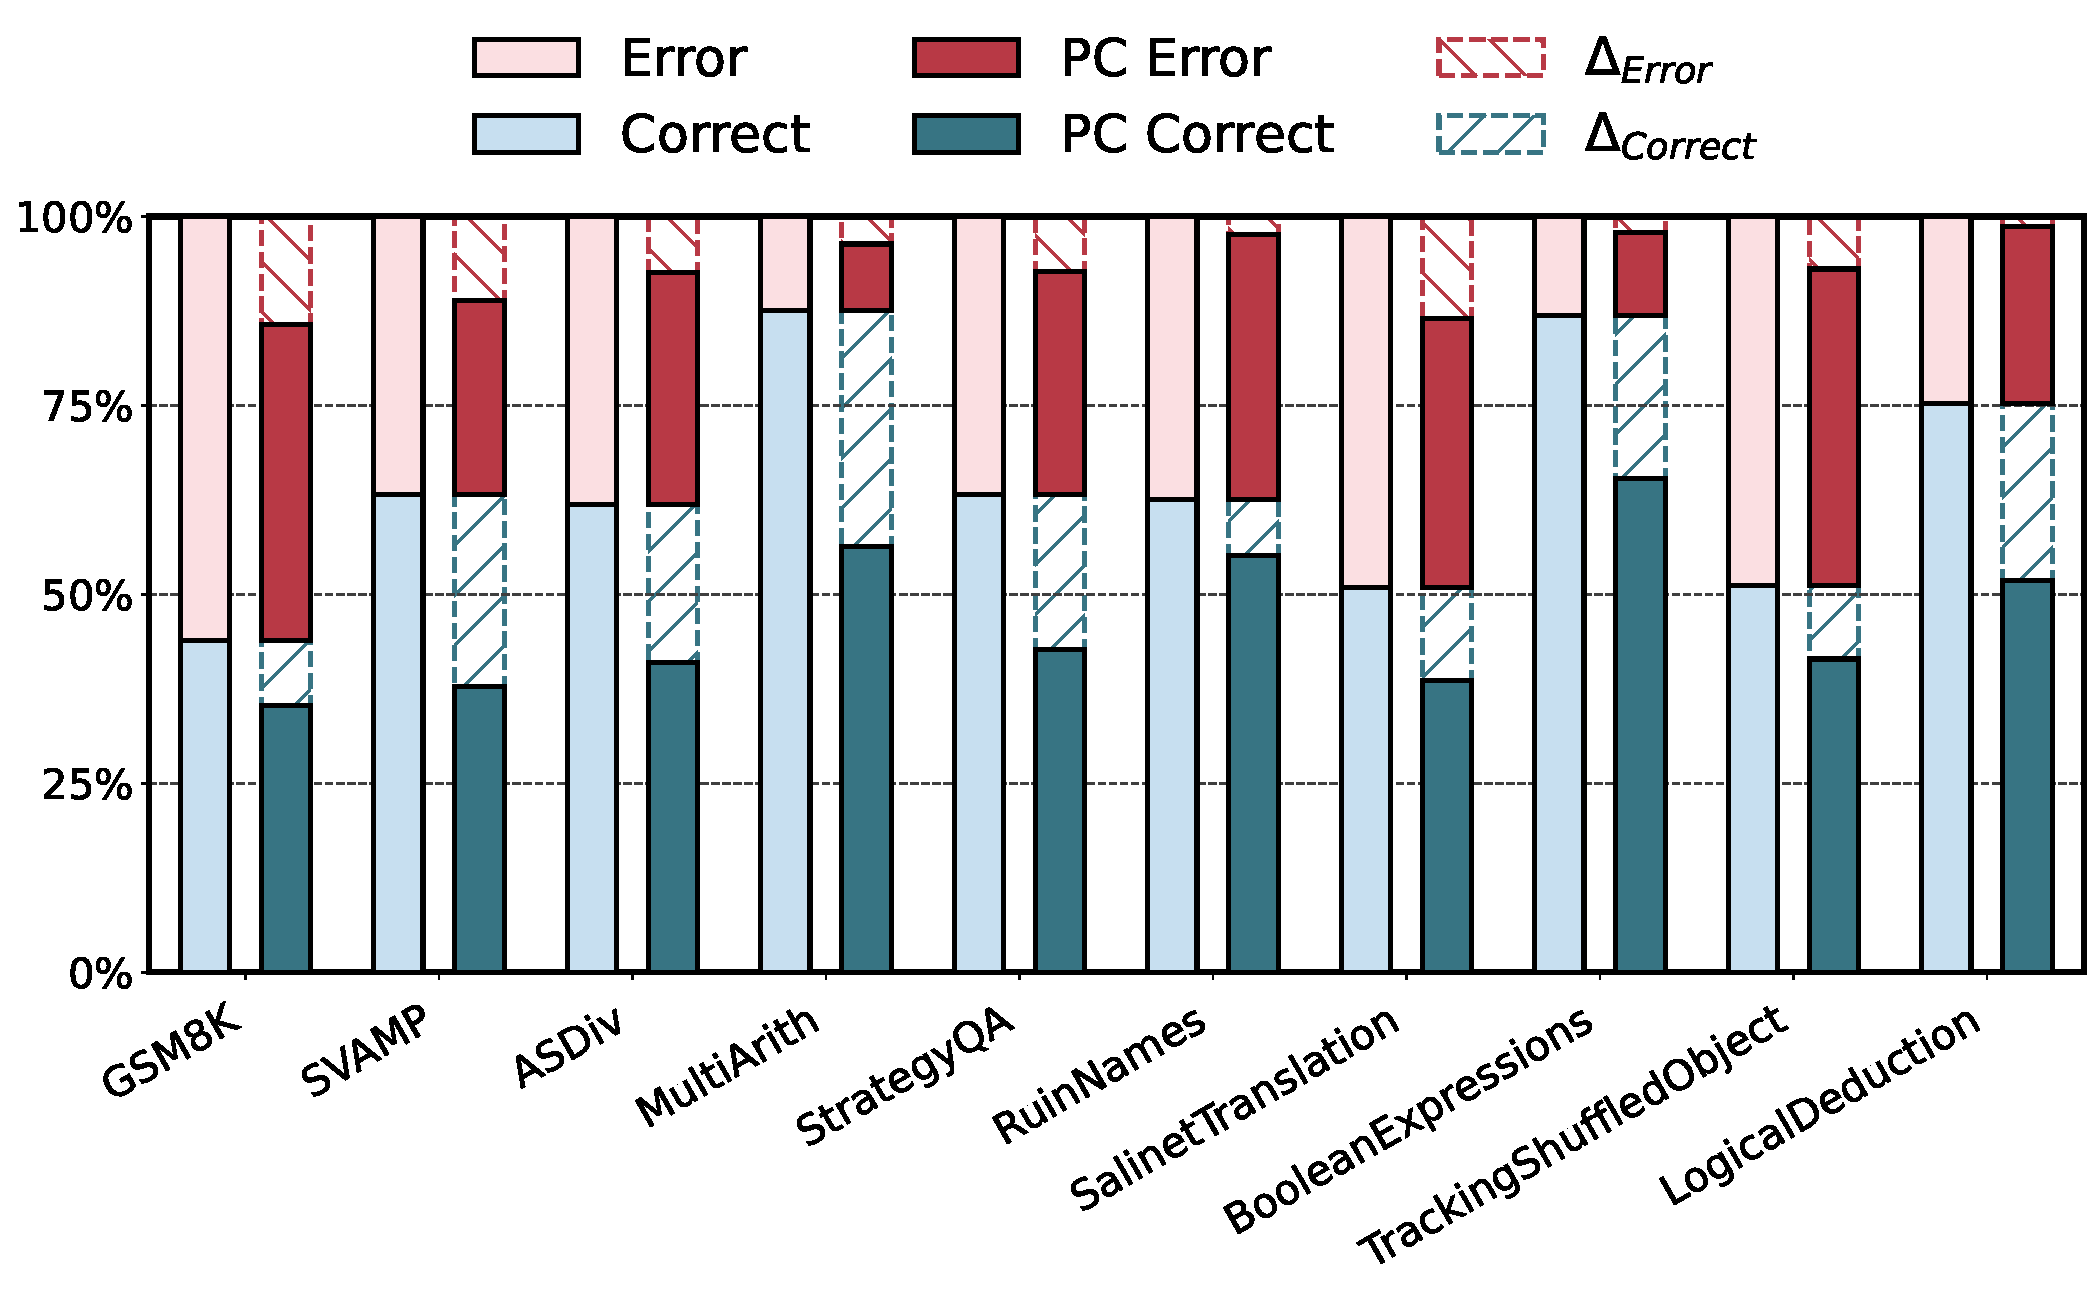
\includegraphics[width=\linewidth]{figs/supp_token_allocation_comparison.pdf}
\caption{Token allocation in the initial sentence-level experiments. Light bars show SC, dark bars show PC, and hatched areas indicate reductions relative to SC. Correct and Error classify trajectories by their final answers, not individual tokens.}
\label{fig:historical_motivation}
\end{figure}

We also examined whether answer agreement could guide prefix reuse. Figure~\ref{fig:sentence_agreement} shows that stronger agreement after ten self-consistency trajectories is associated with correct answers across several tasks. Figure~\ref{fig:sentence_agreement_final} compares the final distributions on GSM8K, where sentence-level reuse produces more concentrated agreement. Incorrect answers nevertheless occur at high agreement. These observations motivated agreement-guided control, but not the interpretation of agreement as a correctness certificate.

\begin{figure}[!htbp]
\centering
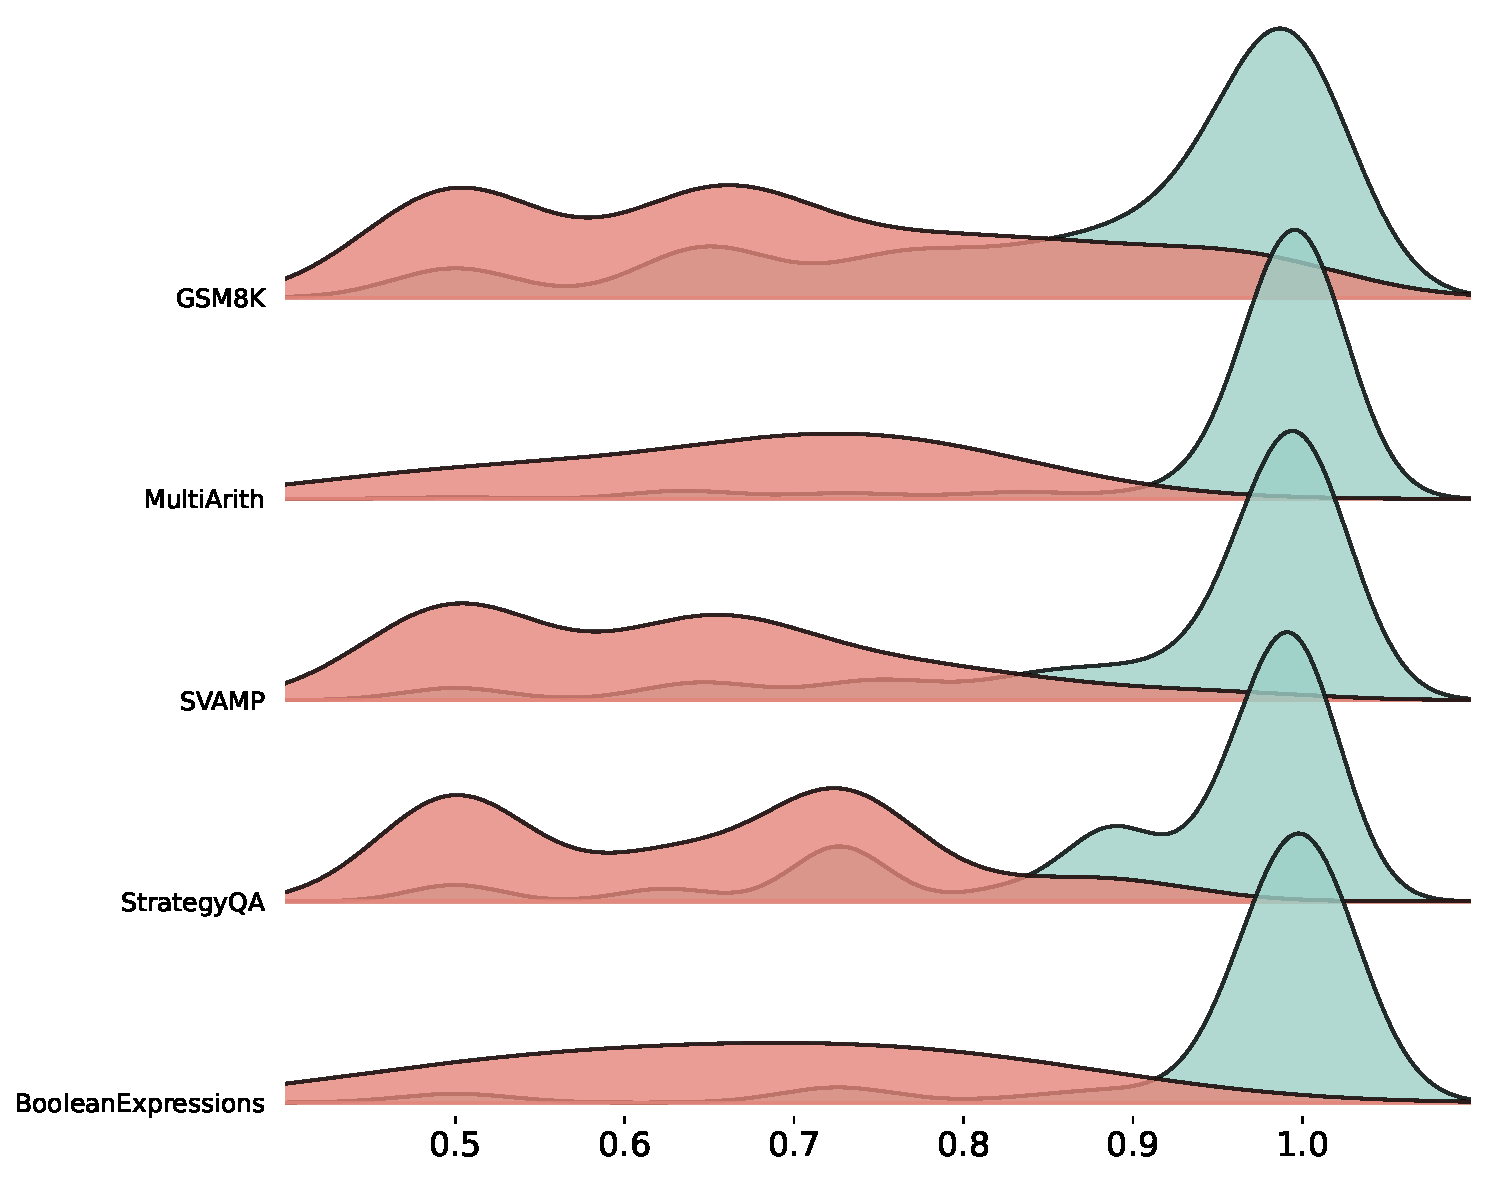
\includegraphics[width=0.62\linewidth]{figs/supp_agreement_by_task.pdf}
\caption{Answer agreement after ten SC trajectories in the initial experiments. Green and red show the distributions for correct and incorrect answers, respectively.}
\label{fig:sentence_agreement}
\end{figure}

\begin{figure}[!htbp]
\centering
\begin{minipage}[t]{0.48\linewidth}
\centering
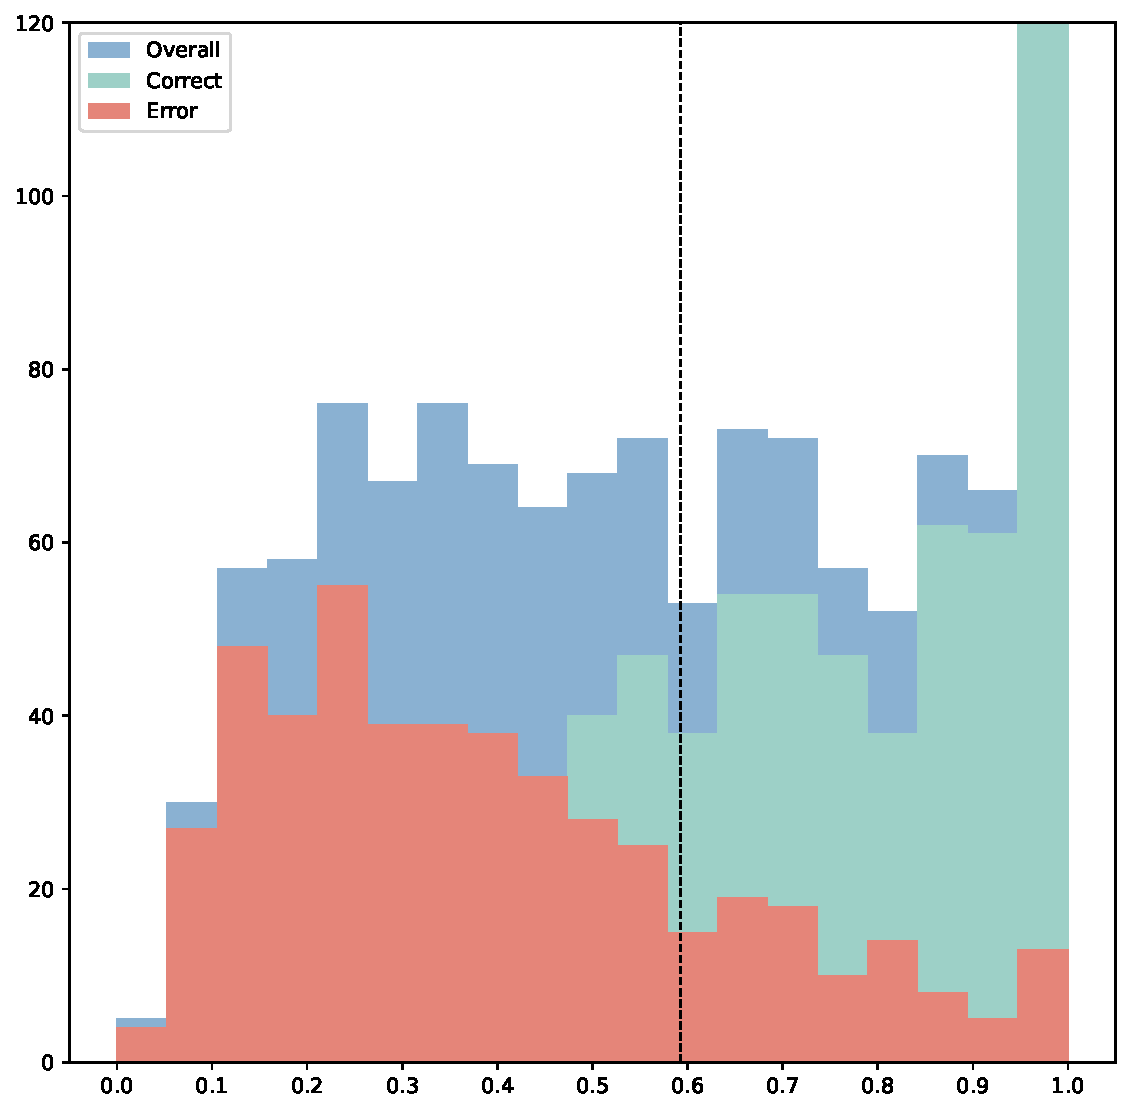
\includegraphics[width=\linewidth]{figs/supp_agreement_sc.pdf}\\[4pt]
{\small (a) Self-consistency}
\end{minipage}\hfill
\begin{minipage}[t]{0.48\linewidth}
\centering
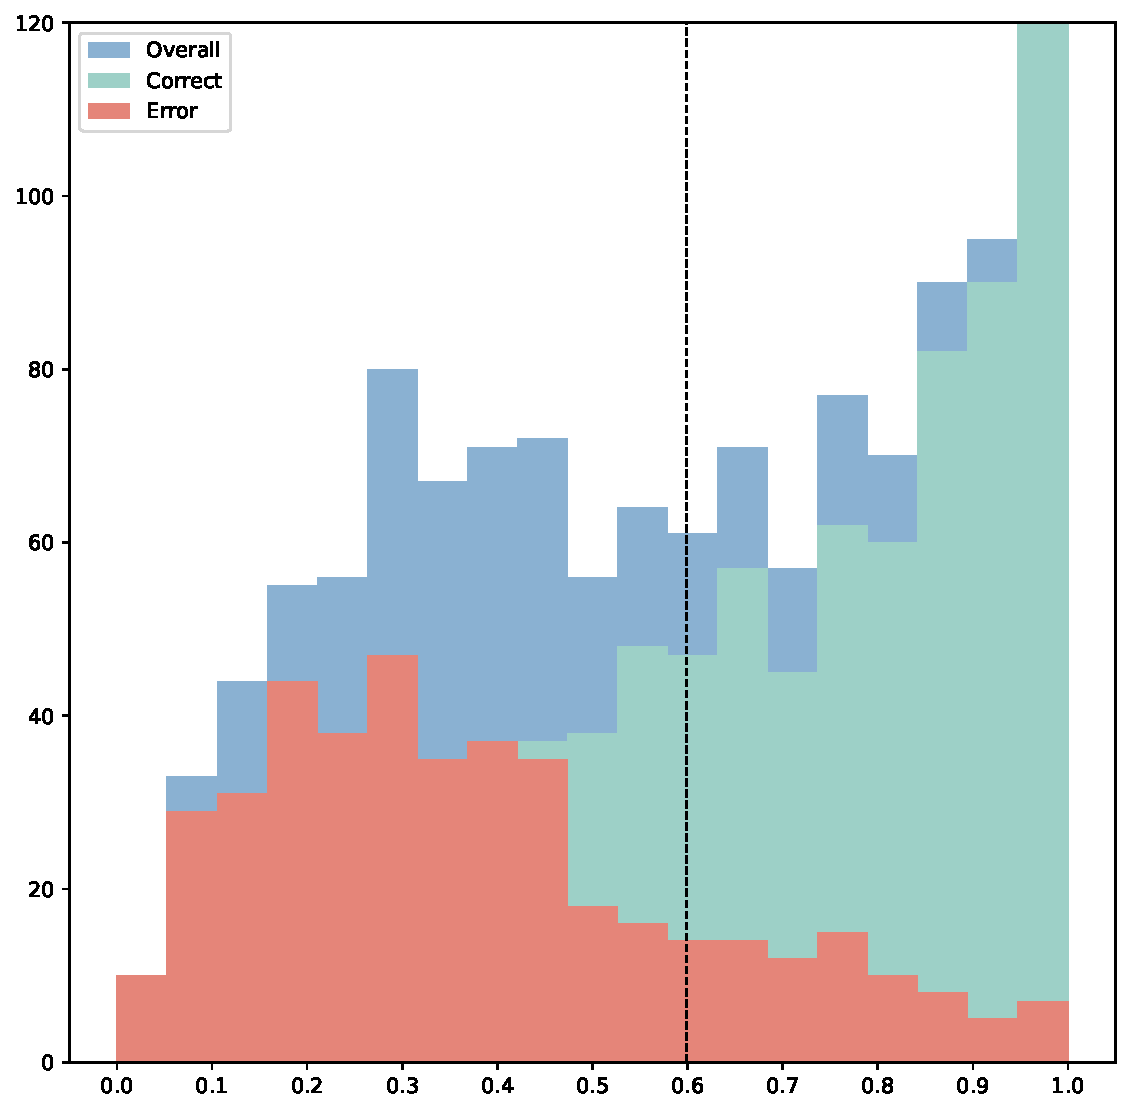
\includegraphics[width=\linewidth]{figs/supp_agreement_pc.pdf}\\[4pt]
{\small (b) Path-consistency}
\end{minipage}
\caption{Final answer agreement on GSM8K in the sentence-level experiments, with $C=0.8$ for PC. Blue shows all questions, green correct answers, and red incorrect answers. The panels use the same axis scales.}
\label{fig:sentence_agreement_final}
\end{figure}

\subsection{Illustrative reasoning trajectories}
Table~\ref{tab:sentence_example} illustrates progressive sentence-prefix reuse. Inherited text is retained while the newly generated suffix becomes shorter. It shows how the initial approach reused complete reasoning steps, complementing the token-fraction example of the current method in Table~\ref{tab:prefix_case}.

\begin{table}[!htbp]
\centering\small
\caption{A sentence-level prefix example. Black text is reused and blue text is newly generated.}
\label{tab:sentence_example}
\begin{tabularx}{\linewidth}{@{}lX@{}}
\toprule
Question & A robe takes 2 bolts of blue fiber and half that much white fiber. How many bolts in total does it take?\\
\midrule
No prefix & \textcolor{blue}{To make a robe, we need 2 bolts of blue fiber and half that much white fiber. We can write this as 2 + 1/2 * 2. Now 1/2 * 2 = 1, so the equation becomes 2 + 1 = 3. The answer is 3.}\\
\midrule
Level 1 & To make a robe, we need 2 bolts of blue fiber and half that much white fiber. \textcolor{blue}{2 * 1/2 = 1 bolt of white fiber. 2 + 1 = 3 bolts in total. The answer is 3.}\\
\midrule
Level 2 & To make a robe, we need 2 bolts of blue fiber and half that much white fiber. 2 * 1/2 = 1 bolt of white fiber. \textcolor{blue}{1 + 2 = 3 bolts in total. The answer is 3.}\\
\midrule
Level 3 & To make a robe, we need 2 bolts of blue fiber and half that much white fiber. 2 * 1/2 = 1 bolt of white fiber. 1 + 2 = 3 bolts in total. \textcolor{blue}{The answer is 3.}\\
\bottomrule
\end{tabularx}
\end{table}

A second example asks how much water remains after two girls each receive one sixth of 24 liters and a boy receives 6 liters. The correct answer is 10 liters. Table~\ref{tab:sentence_recovery} summarizes the Llama-3.2-1B-Instruct trajectories. Prefix levels increase and later return to zero; the final vote is correct despite earlier disagreement. The example shows that a return to unprefixed sampling can occur, but does not prove that the reused text was wrong or that recovery caused the correct final answer.

\begin{table}[!htbp]
\centering\small
\caption{Window-level summary of the water-allocation example. Tokens are the total newly generated tokens in each five-trajectory window. The recorded final answer is 10; answers 10 and 14 each receive seven votes.}
\label{tab:sentence_recovery}
\begin{tabular}{@{}rrlr@{}}
\toprule
Window & Prefix level & Sampled answers & Tokens\\
\midrule
1 & 0 & 8, 10, 14, 14, 14 & 383\\
2 & 1 & 2, 14, 14, 10, 16 & 283\\
3 & 2 & 10, 10, 10, 10, 12 & 89\\
4 & 0 & 16, 14, 2, 10, 14 & 380\\
\bottomrule
\end{tabular}
\end{table}

\subsection{Controller overhead and parallelism}
The sentence-level Llama-3-8B/GSM8K measurements in Table~\ref{tab:sentence_overhead} show that agreement evaluation and prefix selection take little time relative to model generation in that setting. They do not measure the full controller cost of the current method, which also ranks local confidence scores and manages trial and recovery.

\begin{table}[!htbp]
\centering\small
\caption{Controller timing in the supplementary 20-trajectory Llama-3-8B/GSM8K evaluation. Percentages are relative to the reported model-generation time.}
\label{tab:sentence_overhead}
\begin{tabular}{@{}lrr@{}}
\toprule
Component & Time (s) & Relative time (\%)\\
\midrule
Model generation & 2.2 & 100\\
Answer agreement evaluation & 0.000096 & 0.0044\\
Prefix construction & 0.00013 & 0.0059\\
\bottomrule
\end{tabular}
\end{table}

Windowed reuse also constrains parallelism. Trajectories within a window can run concurrently, but the next window depends on the preceding answers and prefix decision. Larger windows allow more concurrent generation, whereas smaller windows offer more frequent opportunities to extend a prefix. Token savings therefore need not translate into proportional latency reductions, especially when independent self-consistency trajectories can be served with greater parallelism.

\subsection{Prompt structure and scope}
The sentence-level experiments use few-shot demonstrations containing a question, reasoning, and final answer. Table~\ref{tab:sentence_prompts} summarizes their format without repeating the full demonstration sets. These prompts are distinct from the chat and thinking interfaces used in the main evaluation.
% Citation placeholders for the original CoT demonstrations and BIG-Bench Hard prompts.
% Full source demonstrations remain in paper/NIPS/appendix.tex.
\begin{table}[!htbp]
\centering\small
\caption{Prompt structure for the supplementary sentence-level experiments. Demonstrations supply intermediate reasoning followed by an explicit final answer.}
\label{tab:sentence_prompts}
\begin{tabularx}{\linewidth}{@{}lXX@{}}
\toprule
Task family & Demonstration content & Answer format\\
\midrule
Arithmetic reasoning & Arithmetic steps leading to a numerical result & The answer is [number].\\
StrategyQA & Short factual reasoning for a yes/no question & The answer is yes/no.\\
Ruin Names & Comparison of candidate humorous edits & The answer is [option].\\
Salient Translation & Comparison of a source sentence and its translation & The answer is [error-type option].\\
Boolean Expressions & Evaluation using logical operator precedence & The answer is True/False.\\
Tracking Shuffled Objects & State updates after successive swaps & The answer is [option].\\
Logical Deduction & Ordering objects from the supplied constraints & The answer is [option].\\
\bottomrule
\end{tabularx}
\end{table}

\paragraph{Implications for the current method.}
The initial experiments showed that reusing intermediate reasoning can shorten later trajectories across several short-chain tasks. They also exposed the trade-off between more aggressive reuse and accuracy preservation. The current method builds on this idea with one continuous shared prefix per window, a token-fraction length policy, local confidence selection, and explicit trial and recovery. The earlier results motivate this design direction; the experiments in Section~\ref{sec:evaluation} evaluate the resulting method.

These experiments do not train or modify the evaluated models. Their computational benefits and failure modes depend on the available reusable reasoning, the agreement threshold, and the generation interface. Reducing inference cost may improve accessibility but can also reduce the cost of harmful uses of the underlying models. Dataset text and model weights remain subject to their providers' terms and are not redistributed with the supplementary results.
